\section{Use of the Operators in a Surveillance Camera System}
In this section, we use the operators previously defined to coordinate the heterogeneous models of a surveillance camera system. To do so, we propose to use \bflow to specify how the operators are applied on the models that compose the surveillance camera system. In the following, we first present the \bflow specification, and then we use it to coordinate the system. 

To coordinate the surveillance camera system, we use \bflow to specify how the operators \emph{SyncFSMEventsAndSignals}, \emph{StartActivityWhenEnter} and \emph{AtomicActivity} are applied between the different models. We define a \bflow specification named \emph{CameraSystem} (Listing~\ref{lst:bflowcamerasystem}: line 1) that begins by importing the \bcool specification (Listing~\ref{lst:bflowcamerasystem}: line 2), and then, it specifies the models to be coordinated (Listing~\ref{lst:bflowcamerasystem}: line 3 to 6). The specification contains a \emph{Flow} that defines which operator is applied and on which models. We describe in turn what operator is applied and what coordination is generated.

First, the operator SyncFSMEventsAndSignals has to be applied between the activity BatterySensor and the TFSM CameraEncoderControl (Listing~\ref{lst:bflowcamerasystem}: line 8). This results in the synchronization of the corresponding Signal and FSMEvent by relying on theirs names. The application of this operator results in \emph{two} instances of the \ccsl relation rendezvous between the \mse \emph{BatteryIsHigh:signalOccurs} and \emph{BatteryisHigh:occurs}; and the \mse \emph{BatteryIsLow:signalOccurs} and \emph{BatteryIsLow:signalOccurs}. 

Then, the operator StartActivityWhenEnter has to be applied between the TFSM CameraEncoderControl and the activity doJPEG (Listing~\ref{lst:bflowcamerasystem}: line 9), and between the TFSM and the activity doJPEG2000 (Listing~\ref{lst:bflowcamerasystem}: line 10). This results in a synchronization between the entering and leaving of the states JPEGEncoder and JPEG2000Encoder, and the execution of the activities doJPEG and doJPEG2000. The application of this operator results in \emph{two} instances of the \moccml relation ExecuteActivityNonPeemptive between the \mse \emph{doJPEG:startActivity}, \emph{doJPEG:finishActivity}, \emph{JPEGEncoder:entering} and \emph{JPEGEncoder:leaving}; and the \mse \emph{doJPEG2000:startActivity}, \emph{doJPEG2000:finishActivity}, \emph{JPEG2000Encoder:entering} and \emph{JPEG2000Encoder:leaving}.   

Finally, to coordinate the time between the TFSM and the activities, the operator AtomicActivity has to be applied between the TFSM CameraEncoderControl and each activity (Listing~\ref{lst:bflowcamerasystem}: line 11 and 12). This results in a synchronization between the local clock \emph{ms} of the TFSM CameraEncoderControl and the execution of the activities. The application of this operator results in \emph{two} instances of \moccml relation AtomicActivity between the \mse \emph{doJPEG2000:startActivity}, \emph{doJPEG2000:finishActivity} and \emph{ms:ticks}; and the \mse \emph{doJPEG:startActivity}, \emph{doJPEG:finishActivity} and \emph{ms:ticks}.


\begin{lstlisting}[language=bflow,
caption={\bflow specification for the Surveillance Camera System},
label={lst:bflowcamerasystem}, 
basicstyle=\scriptsize\ttfamily, backgroundcolor=\color{LGrey}, numbers=left, xleftmargin=2pt]
BCOoLFlow CameraSystem
ImportBCOoL  "TFSMAndActivity.bcool" ;
Model BatterySensor "batterysensor.ad"
Model CameraEncoderControl "cameraencodercontrol.tfsm"
Model doJPEG "doJPEG.ad"
Model doJPEG2000 "doJPEG2000.ad"
Flow 
	applies SyncFSMEventsAndSignals between (BatterySensor, CameraEncoderControl);
	applies StartActivityWhenEnter between (CameraEncoderControl, doJPEG);
	applies StartActivityWhenEnter between (CameraEncoderControl, doJPEG2000);
	applies AtomicActivity between (CameraEncoderControl, doJPEG);		
	applies AtomicActivity between (CameraEncoderControl, doJPEG2000);		
end Flow;
\end{lstlisting}

The resulting model of coordination is thus composed of six relations, \ie two \ccsl relations and four \moccml relations. In the modeling workbench, we use the \bflow specification together with the Gemoc Coordinated Execution Engine to execute the coordinated system. Figure~\ref{fig:studiocamera} illustrates the coordinated execution of the models. In the figure, four Gemoc execution engines are launched that correspond with the four models of the surveillance system. Also, one coordinated execution engine is launched that corresponds with the coordination between these models. 

		\begin{figure}[h]
			\center
			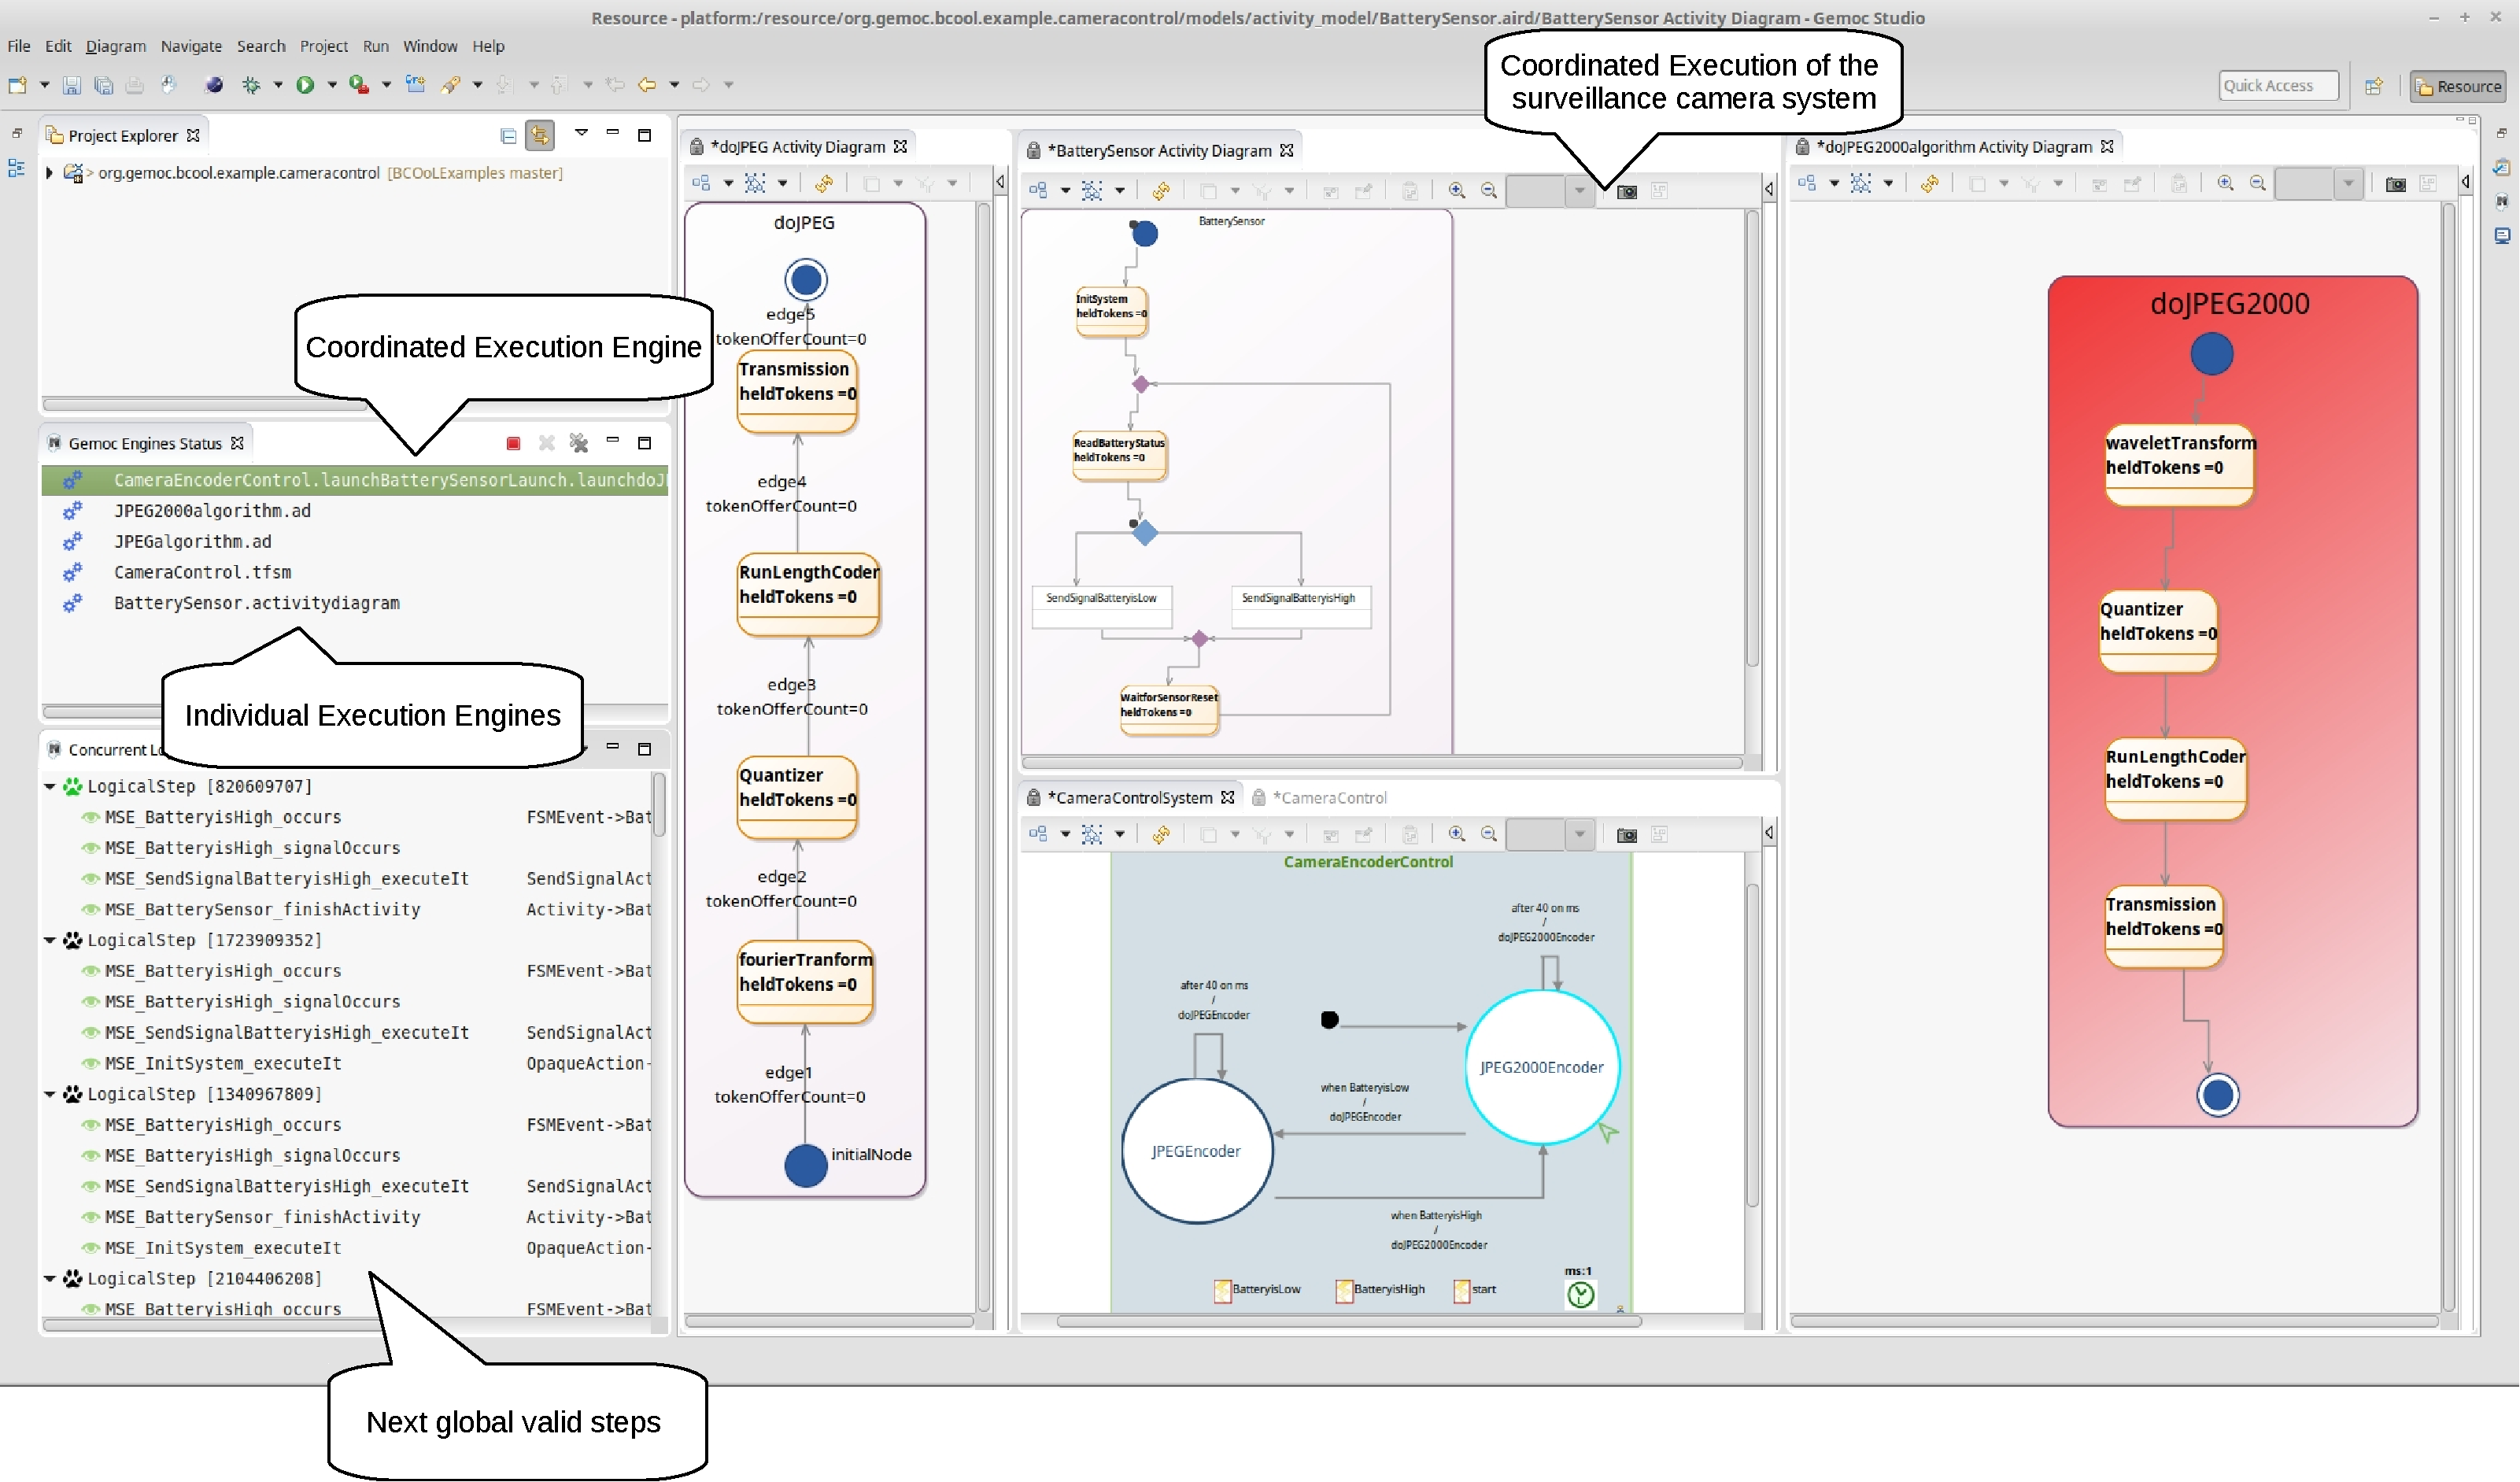
\includegraphics[width=.9\columnwidth]{examples/figs/screenshot}
			\caption{Coordinate execution of the models of the surveillance camera system by using the Gemoc studio}
			\label{fig:studiocamera}
		\end{figure}


Figure~\ref{fig:camerasystem} illustrates the partial timing output of the execution of the camera. As a result of the coordination, the \mse \emph{BatteryisHigh:occurs} and \emph{BatteryisHigh:signalOccurs} are strongly synchronized (in red in Figure~\ref{fig:camerasystem}). When the camera entered into the JPEG2000Encoder state (in magenta in Figure~\ref{fig:camerasystem}), the activity doJPEG2000 executes and the time in the TFSM does not elapse (in cyan in Figure~\ref{fig:camerasystem}). Only after the activity has finished, the time can elapse thus the \mse \emph{ms:ticks} is allowed to tick. Also, only after the activity has finished the state is allowed to be left. In this example, the state-space graph of the coordinated system is not finite. This makes that the state-space graph of the coordinated system is not computable. Thus, we could not get results on the scheduling state-space of the coordinated system.
	
		\begin{figure}[h]
			\center
			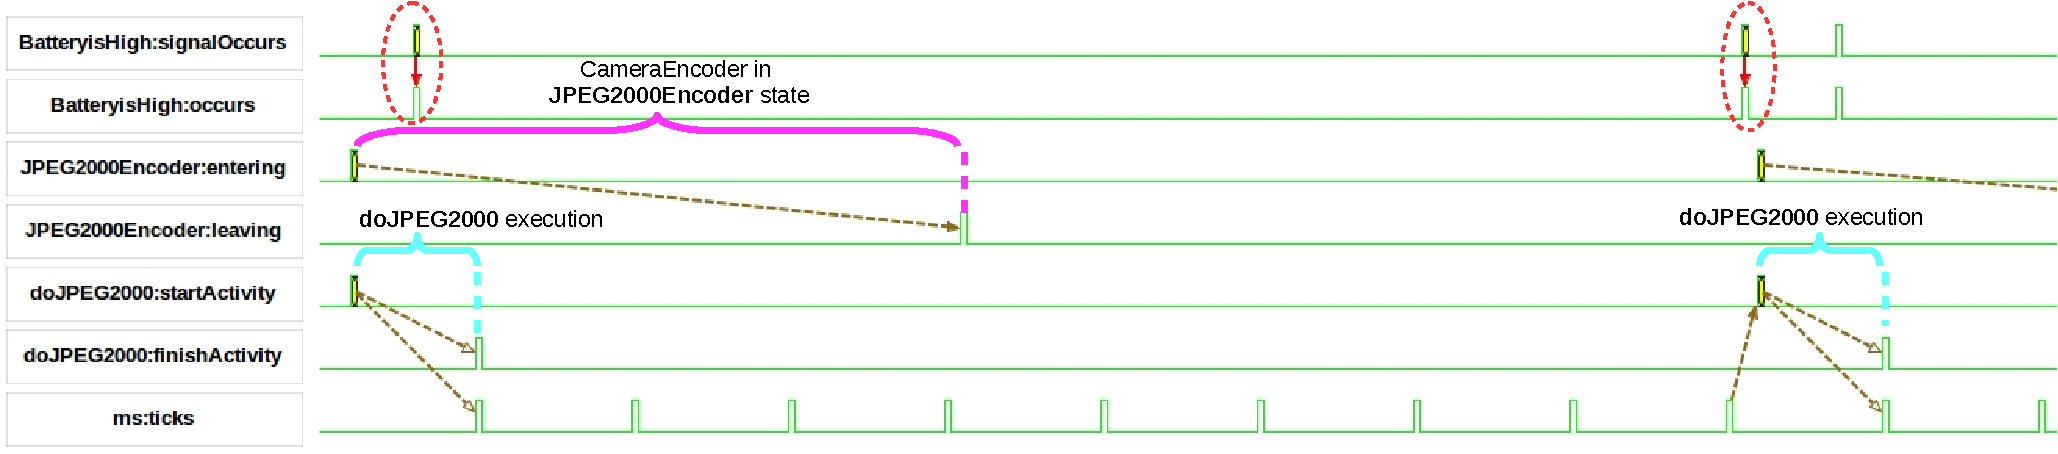
\includegraphics[width=1\columnwidth]{examples/figs/vcdcamera}
			\caption{Partial resulting timing output of the surveillance camera system}
			\label{fig:camerasystem}
		\end{figure}
	
In this section, we have shown the use of \bflow to specify how the operators defined in the previous section are applied between the models of the camera. Then, we used this specification in the modeling workbench to execute and verify the coordinated system. By relying on \ccsl to express the coordination, we could provide execution and verification of the coordinated system. We want to highgligt that in coordination frameworks these tasks are limited since they express the coordination in a GPL like Java in Ptolemy. The reader can find the complete example in the companion website, which contains the models together with a detailed procedure to execute and verify them. In addition, the site includes a video that shows the complete workflow by using the GEMOC studio.

%\todo{We want to highlighted that given the constrainst that we fixed and since all the states in the Camera are represented by activities, this makes the time not elapse at all. In the simulation, we only coordinated one of the activities, thus when the TFSM is in the other state the time is allowed to pass. The main drawback of this, is, since the activity as atomic, the time not elapse, this prevents the use of the timing transitions in the TFSM. In fact, there is non such a constrains, the time may elapse after the finishing of the activity and before the starting of it. However, this is hard to see that in the simulation, politic of the simulation?}

%In this subsection, we have presented the \bflow specification for the coordination of the surveillance camera system. The \bflow specification defines how to build the coordination model for the camera system by relying on the operators previously defined.
%the operator SyncProdut must be applied one time to coordinate the models … Then, the operators startActivityWhenEnter and AtomicActivity must be applied twice, one time for each activity. This specification is only for one camera which is composed by three models. However, this can be extended for N camera by modifying the bflow. 

	
	
	